This section covers the background of the current resource cost analysis,
with a 
motivating example.
This example shows that the traditional way fails to give a tight bound on the program's resource cost.
% similarity between general and the program's adaptivity accumulation,
Then, this section covers the proposed methodology I plan to adopt for an accurate full-Spectrum
analysis on 
% the general resource cost analysis.
the program's resource cost.
% \section{Introduction}
% \label{sec:generalcost-backgroung}
% Through observation in following example, the heap resource consumption during the program 
% execution is accumulating in the same way as the program's adaptivity. 
% More specifically in Example~\ref{}Specifically, in line 5 
% where the list is re-written and the heap consumption is decreased implicitly. 
% This implicit decrease 
% of the cost works exactly the same as program's adaptivity decrease.
% \\
% This motivates the generalization of the analysis framework onto the program's resource cost analysis. Use this framework,
% I will give
% a more accurate resource cost estimation 
% by taking the program's implicit resource cost into consideration, comparing 
% to the worst case cost analysis in traditional way.
% \\
\subsection{Background and Related Work}
There are mainly two categories of methodology in the static program resource cost analysis areas, 
through type-system based  and data-flow/control-flow analysis based. 
They can be summarized briefly as follows, but to the best of my knowledge,
all these works in the two categories fail to recognize the case where program resource consumption is decreased implicitly.
 \paragraph*{Type-System Based}
Existing
static program analysis based type-system are mainly through 
effect systems, 
% control-flow analysis, and data-flow analysis~\cite{ryder1988incremental}. 
% The idea of statically estimating a sound upper bound for the adaptivity from the semantics is indirectly inspired from prior work on cost analysis via effect systems~\cite{cciccek2017relational,radivcek2017monadic,qu2019relational}. The idea of defining adaptivity using data flow is inspired by the work of graded 
Hoare logic~\cite{gaboardi2021graded}, and amortized type system~\cite{hoffmann_jost_2022}.
%
In these systems, the cost are accumulating through the type induction. 
The only way to save the cost into the potential
type, as in~\cite{GustafssonEL05} and \cite{hoffmann_jost_2022}, 
is through explicit abstraction or data structure de-allocation.
That is to say, they cannot deal with the case where the cost (for example the adaptivity) decreases when there isn't a dependency relation between variables.
\paragraph*{Data-flow/Control-flow Analysis Based}
Existing static program analysis works via the control flow or data flow analysis 
in program resource cost analysis 
mainly falls into two areas, the program complexity analysis and worst case execution time analysis. 
They are focusing on analyzing the cost of the entire program. 
The techniques are based on
type system~\cite{CicekBG0H17, RajaniG0021}, Hoare logic~\cite{CarbonneauxHS15}, abstract interpretation~\cite{GustafssonEL05, HumenbergerJK18},
invariant generation through cost equations or ranking functions~\cite{BrockschmidtEFFG16,AlbertAGP08,AliasDFG10,Flores-MontoyaH14}
or a combination of program abstraction and invariant inferring~\cite{GulwaniZ10, SinnZV17,GulwaniJK09}.
In general, these techniques give the approximated upper bound of the program's total running time or resource cost.
However, they failed to consider the case where the program's cost could decrease when there isn't a dependency relation between variables.

\subsection{Motivation}
\label{subsubsec:furthers-cost-example}
As shown in the Example~\ref{ex:heapcost} above, the heap resource consumption during the program 
execution is accumulating in the same way as the program's adaptivity. 
Specifically, in line : 6 and line :  9
the list assigned to $x$ and $y$ is re-written instead of accumulated.
So the heap consumption is in the loop isn't accumulated recursively, which is exactly
the same as the case where the adaptivity isn't accumulated because of non-dependency between variables.
In other words, these operations in above cases imply implicit cost decreases 
which are all considered as increases in traditional resource analysis 
method.
The following example in Example~\ref{ex:heapcost} shows that in general 
resource cost analysis, the $\THESYSTEM$  can give a better cost upper bound than the traditional 
data-flow or control-flow analysis.
% program shown in Figure~\ref{fig:heapcost_example.tex} shows the similarity
% between the adaptivity and cost estimation.
\begin{example}[Resource Cost Example]
  \label{ex:heapcost}
The example program shown in Figure~\ref{fig:heapcost_example.tex} shows the similarity
between the adaptivity and cost estimation.

In order to estimate the worst case heap cost in this program, I analyse the length 
of the list assigned to $x$ and $y$ in line:6 and line : 9 of this program, through $\THESYSTEM$.
Then,  $\THESYSTEM$ computes approximation
of heap resource cost by searching for longest finite walk.
\\
Specifically as follows, 
$\THESYSTEM$ first constructs the program-based execution as in Figure~\ref{fig:heapcost_example.tex},
with weight on each vertex. (The query annotation in the graph is omitted, which isn't useful in analysing the 
list length).
Then $\THESYSTEM$ compute the longest restricted finite walk on this graph.
\\
In order to compute the bound for heap resource cost, the length of walk takes the non-query vertices into consideration as 
well. 

%  largest length of $x$ and $y$ 
% search for a path: $y^6 \to y^6$, and compute the adaptivity for this path as 
% $k$.
% Notice here, another special operation I have in the second branch is Non-updating of
% % Non-updating the 
% $\kw{querynum}$ and $\kw{flowcapacity}$.
% This guarantees both the accuracy and the soundness.
% Specifically,
% % because a second visiting of the same vertex 
% if this vertex is visited, it indicates that a cycle is monitored and  
% % indicates there is a cycle goes back to this vertex, 
% the traversing on this cycle is finished by going back to this vertex.
% %
% % then, when 
% When I continuously search for walks heading out of this vertex, 
% the minimum weight on this cycle does not affect the walks going out of this vertex that not pass this cycle.
% However, if I keep recording the minimum weight, then we
% %  are restricting 
% restrict the visiting times of vertices on a walk by
% using the minimum weight of vertices not on this walk.
% %  , it is unsound anymore.
% Then, it is obviously that this leads to unsoundness.
% If I update the $\kw{flowcapacity}[y^6]$ as $k$ after visiting $y^6$ the second time 
% on this walk,
% % the walk $y^6 \to y^6$,
% and continuously visit $x^9$,
% then the $\kw{flowcapacity[k]}$ is 
% updated as $\min(k, k^2)$.
% So
% %  which 
% % restricting 
% the visiting times of $x^9$ is restricted by $k$ on the walk $y^6 \to y^6 \to x^9$.
% This restriction excludes the finite walk $y^6 \to y^6 \to x^9 \to x^9$ where $y^6$ and $x^9$ visited by $k^2$ times
% in the computation. 
% However, the finite walk $y^6 \to y^6 \to x^9 \to x^9$ where $y^6$ is visited $k$ times and $x^9$ $k^2$ times is 
% a qualified walk, and exactly the longest walk I aim to find. So, by Non-updating the $\kw{flowcapacity}$ after 
% visiting $y$ again, I guarantee that the visiting times og vertices on every searched walk will not be restricted by weights not on this walk,
% i.e., the soundness.
% \\
% In the last line of this dfs algorithm, line: 16, it returns the adaptivity heading out from its input vertex.
% \\
% By applying this deep first search strategy on every vertex on this SCC, 
% I compute the adaptivity of this SCC by taking the maximum 
% % adaptivity reaching every vertex on this SCC.
% value over every vertex.
%
As a result,
the largest heap resource consumed in total, by $y$ and $x$ together computed from the $\THESYSTEM$ is $1 + k^2 + k$.
Comparing to $k + k^2 + k^3$ estimated as  the longest weight path from traditional CFL-reachability method, 
$\THESYSTEM$ analysis result improves the accuracy by $O(n)$.

% Look at a Nested While Loop example program in Figure~\ref{fig:heapcost_example.tex}.
% Specifically,
% % because a second visiting of the same vertex 
% if this vertex is visited, it indicates that a cycle is monitored and  
% % indicates there is a cycle goes back to this vertex, 
% the traversing on this cycle is finished by going back to this vertex.
% %
% % then, when 
% When I continuously search for walks heading out of this vertex, 
% the minimum weight on this cycle does not affect the walks going out of this vertex that not pass this cycle.
% However, if I keep recording the minimum weight, then we
% %  are restricting 
% restrict the visiting times of vertices on a walk by
%  using the minimum weight of vertices not on this walk.
% %  , it is unsound anymore.
% Then, it is obviously that this leads to unsoundness.
 %
  %
  \begin{figure}
    \centering
    {
      % \footnotesize
    \begin{subfigure}{.4\textwidth}
    \begin{centering}
    % 
    $ 
    \begin{array}{l}
      \kw{nestedWhileMultiVarRecAcross}(k) \triangleq \\
      \clabel{\assign{i}{k} }^{0} ; 
      \clabel{ \assign{x}{[]}}^{1} ; 
      \clabel{ \assign{y}{[]}}^{2} ; \\
          \ewhile ~ \clabel{i > 0}^{3} ~ \edo ~ \\
          \Big(
           \clabel{\assign{i}{i-1}}^{4} ;
           \clabel{\assign{j}{k}}^{5} ;\\
           \clabel{\assign{x}{1::y} }^{6}  ; \\
           \ewhile ~ \clabel{j > 0}^{7} ~ \edo ~ \\
           \Big(
            \clabel{\assign{j}{j-1}}^{8};
            \clabel{\assign{y}{ 1::x }}^{9}
            \Big) \Big)
      \end{array}
    %       
    $
    \caption{}
    \end{centering}
    \end{subfigure}
    \quad
    \begin{subfigure}{.52\textwidth}
      \begin{centering}
      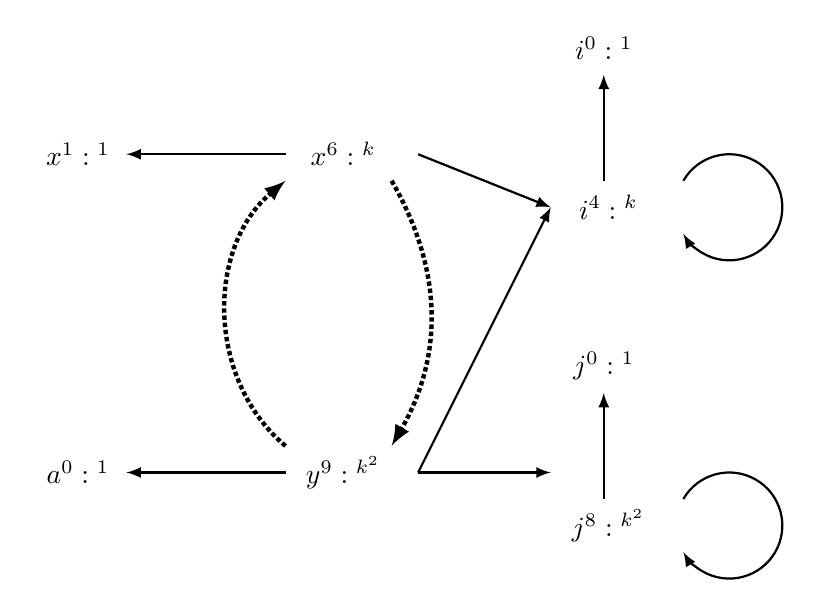
\begin{tikzpicture}[scale=\textwidth/18cm,samples=200]
      % Variables Initialization
      \draw[] (-5, 1) circle (0pt) node{{ $a^0: {}^1$}};
      \draw[] (-5, 7) circle (0pt) node{{ $x^1: {}^{1}$}};
      % Variables Inside the Loop
      \draw[] (0, 7) circle (0pt) node{{ $x^6: {}^{k}$}};
      \draw[] (0, 1) circle (0pt) node{{ $y^9: {}^{k^2}$}};
      % Counter Variables
      \draw[] (5, 9) circle (0pt) node {{$i^0: {}^{1}$}};
      \draw[] (5, 6) circle (0pt) node {{ $i^4: {}^{k}$}};
      \draw[] (5, 3) circle (0pt) node {{$j^0: {}^{1}$}};
      \draw[] (5, 0) circle (0pt) node {{ $j^8: {}^{k^2}$}};
      % Value Dependency Edges:
      \draw[ thick, -latex] (5, 6.5)  --       (5, 8.5) ;
      \draw[ thick, -latex] (5, 0.5)  --       (5, 2.5) ;
      % Value Dependency Edges on Initial Values:
      \draw[ thick, -latex,] (-1, 1)  -- (-4, 1) ;
      \draw[ thick, -latex,] (-1, 7)  -- (-4, 7) ;
      %
      \draw[ ultra thick, -latex, densely dotted,] (-1, 1.5)  to  [out=-220,in=220]  (-1, 6.5);
      % node[left]{\highlight{{$k$}}}
      \draw[ ultra thick, -latex, densely dotted,]  (1, 6.5) to  [out=-60,in=60] (1, 1.5) ;
      % node[right]{\highlight{{$k$}}}
      % Control Dependency
      \draw[ thick, -latex, ] (6.5, 6.5) arc (150:-150:1);
      \draw[ thick, -latex, ] (6.5, 0.5) arc (150:-150:1);
      \draw[ thick,-latex] (1.5, 7)  -- (4, 6) ;
      \draw[ thick,-latex] (1.5, 1)  -- (4, 6) ;
      \draw[ thick,-latex] (1.5, 1)  -- (4, 1) ;
   \end{tikzpicture}
   \caption{}
      \end{centering}
      \end{subfigure}
    }
     \caption{(a) Nested While Loop Example, (b) Execution-Based Dependency Graph, (c) The Static Program-Based Dependency graph.}
    \label{fig:heapcost_example.tex}
    \vspace{-0.5cm}
    \end{figure}
  \end{example}


\subsection{Analysis Framework via $\THESYSTEM$ Overview}
\label{sec:generalcost-methodology}
As discussed in Section~\ref{subsubsec:furthers-cost-example}
% shown in the Example~\ref{ex:heapcost} above, the heap resource consumption during the program 
% execution is accumulating in the same way as the program's adaptivity. 
% Specifically, in line : 6 and line :  9
% the list assigned to $x$ and $y$ is re-written instead of accumulated.
% So the heap consumption is in the loop isn't accumulated recursively, which is exactly
% the same as the case where the adaptivity isn't accumulated because of non-dependency between variables.
% In other words, these operations in above cases imply implicit cost decreases 
% which are all considered as increases in traditional resource analysis 
% method.
% In other wor decreased implicitly. 
% This implicit decrease 
% of the cost works exactly the same as program's adaptivity decrease.
according to this high similarity between the program's resource cost and the 
program's adaptivity property, I adopt the similar analysis procedure as in Section~\ref{ch:dynamic} and 
Section~\ref{ch:static},
and generalize 
% This motivates the generalization of 
% the analysis
$\THESYSTEM$ framework onto the general resource cost analysis. 
Based this framework,
I will give
a more accurate resource cost estimation by taking the program's implicit resource cost into consideration, comparing 
to the worst case cost analysis in traditional way. Specifically as follows:
% \\
\paragraph*{Language Generalization} Since the interested property 
to be analysed isn't the \emph{adaptivity},
the {\tt Query While} Language will be generalized into standard while language with inter-procedure function call.
% \\
\paragraph*{Resource Cost Formalization through Execution-Based Analysis} 
Formalize the program resource cost through an execution-based program analysis as in Section~\ref{sec:dynamic}.
In this formalization, instead of formalize the intuitive \emph{adaptive}, the resource cost will be the
target quantitative property of program.
% \\
\paragraph*{Resource Cost Estimation through Generalized $\THESYSTEM$}
According to this high similarity between the program's resource cost and the 
program's adaptivity property, the static program analysis for the resource cost property will 
be performed on a generalized  $\THESYSTEM$.  $\THESYSTEM$ will be generalized specifically as follows:
% \\
% 1.
% % the analysis
% $\THESYSTEM$ framework onto the program's resource cost analysis. 
\begin{enumerate}
    \item The analysis processes in first two steps of $\THESYSTEM$ in Section~\ref{sec:static-datadep}
    and Section~\ref{sec:static-reachability} will be adopted exactly the same in the generalized $\THESYSTEM$.
    \item Then, generalized $\THESYSTEM$ will construct a similar program-based dependency graph 
    in the same way as in Section~\ref*{sec:static-adapt}, but without query annotation. 
    \item According to the formalized resource cost quantity from execution-based analysis above,
    generalized $\THESYSTEM$ will add extra annotation on this graph describing this property.
    \item Then, based on the resource cost quantity, the adaptivity quantity in Definition~\ref{def:prog_adapt}
    will be modified for describing this resource cost quantity, through a modified restricted finite walk.
    \item Then in the last step, the adaptivity computation algorithm will be adopted to search for the longest 
    walk under the modified restriction and compute the bound for 
    this resource cost quantity.
\end{enumerate}

% \section{The Heap Cost Analysis as Non-Linear Property}
% \label{sec:generalcost-example}
% The following example in Example~\ref{ex:heapcost} shows that in general 
resource cost analysis, the $\THESYSTEM$  can give a better cost upper bound than the traditional 
data-flow or control-flow analysis.
% program shown in Figure~\ref{fig:heapcost_example.tex} shows the similarity
% between the adaptivity and cost estimation.
\begin{example}[Resource Cost Example]
  \label{ex:heapcost}
The example program shown in Figure~\ref{fig:heapcost_example.tex} shows the similarity
between the adaptivity and cost estimation.

In order to estimate the worst case heap cost in this program, I analyse the length 
of the list assigned to $x$ and $y$ in line:6 and line : 9 of this program, through $\THESYSTEM$.
Then,  $\THESYSTEM$ computes approximation
of heap resource cost by searching for longest finite walk.
\\
Specifically as follows, 
$\THESYSTEM$ first constructs the program-based execution as in Figure~\ref{fig:heapcost_example.tex},
with weight on each vertex. (The query annotation in the graph is omitted, which isn't useful in analysing the 
list length).
Then $\THESYSTEM$ compute the longest restricted finite walk on this graph.
\\
In order to compute the bound for heap resource cost, the length of walk takes the non-query vertices into consideration as 
well. 

%  largest length of $x$ and $y$ 
% search for a path: $y^6 \to y^6$, and compute the adaptivity for this path as 
% $k$.
% Notice here, another special operation I have in the second branch is Non-updating of
% % Non-updating the 
% $\kw{querynum}$ and $\kw{flowcapacity}$.
% This guarantees both the accuracy and the soundness.
% Specifically,
% % because a second visiting of the same vertex 
% if this vertex is visited, it indicates that a cycle is monitored and  
% % indicates there is a cycle goes back to this vertex, 
% the traversing on this cycle is finished by going back to this vertex.
% %
% % then, when 
% When I continuously search for walks heading out of this vertex, 
% the minimum weight on this cycle does not affect the walks going out of this vertex that not pass this cycle.
% However, if I keep recording the minimum weight, then we
% %  are restricting 
% restrict the visiting times of vertices on a walk by
% using the minimum weight of vertices not on this walk.
% %  , it is unsound anymore.
% Then, it is obviously that this leads to unsoundness.
% If I update the $\kw{flowcapacity}[y^6]$ as $k$ after visiting $y^6$ the second time 
% on this walk,
% % the walk $y^6 \to y^6$,
% and continuously visit $x^9$,
% then the $\kw{flowcapacity[k]}$ is 
% updated as $\min(k, k^2)$.
% So
% %  which 
% % restricting 
% the visiting times of $x^9$ is restricted by $k$ on the walk $y^6 \to y^6 \to x^9$.
% This restriction excludes the finite walk $y^6 \to y^6 \to x^9 \to x^9$ where $y^6$ and $x^9$ visited by $k^2$ times
% in the computation. 
% However, the finite walk $y^6 \to y^6 \to x^9 \to x^9$ where $y^6$ is visited $k$ times and $x^9$ $k^2$ times is 
% a qualified walk, and exactly the longest walk I aim to find. So, by Non-updating the $\kw{flowcapacity}$ after 
% visiting $y$ again, I guarantee that the visiting times og vertices on every searched walk will not be restricted by weights not on this walk,
% i.e., the soundness.
% \\
% In the last line of this dfs algorithm, line: 16, it returns the adaptivity heading out from its input vertex.
% \\
% By applying this deep first search strategy on every vertex on this SCC, 
% I compute the adaptivity of this SCC by taking the maximum 
% % adaptivity reaching every vertex on this SCC.
% value over every vertex.
%
As a result,
the largest heap resource consumed in total, by $y$ and $x$ together computed from the $\THESYSTEM$ is $1 + k^2 + k$.
Comparing to $k + k^2 + k^3$ estimated as  the longest weight path from traditional CFL-reachability method, 
$\THESYSTEM$ analysis result improves the accuracy by $O(n)$.

% Look at a Nested While Loop example program in Figure~\ref{fig:heapcost_example.tex}.
% Specifically,
% % because a second visiting of the same vertex 
% if this vertex is visited, it indicates that a cycle is monitored and  
% % indicates there is a cycle goes back to this vertex, 
% the traversing on this cycle is finished by going back to this vertex.
% %
% % then, when 
% When I continuously search for walks heading out of this vertex, 
% the minimum weight on this cycle does not affect the walks going out of this vertex that not pass this cycle.
% However, if I keep recording the minimum weight, then we
% %  are restricting 
% restrict the visiting times of vertices on a walk by
%  using the minimum weight of vertices not on this walk.
% %  , it is unsound anymore.
% Then, it is obviously that this leads to unsoundness.
 %
  %
  \begin{figure}
    \centering
    {
      % \footnotesize
    \begin{subfigure}{.4\textwidth}
    \begin{centering}
    % 
    $ 
    \begin{array}{l}
      \kw{nestedWhileMultiVarRecAcross}(k) \triangleq \\
      \clabel{\assign{i}{k} }^{0} ; 
      \clabel{ \assign{x}{[]}}^{1} ; 
      \clabel{ \assign{y}{[]}}^{2} ; \\
          \ewhile ~ \clabel{i > 0}^{3} ~ \edo ~ \\
          \Big(
           \clabel{\assign{i}{i-1}}^{4} ;
           \clabel{\assign{j}{k}}^{5} ;\\
           \clabel{\assign{x}{1::y} }^{6}  ; \\
           \ewhile ~ \clabel{j > 0}^{7} ~ \edo ~ \\
           \Big(
            \clabel{\assign{j}{j-1}}^{8};
            \clabel{\assign{y}{ 1::x }}^{9}
            \Big) \Big)
      \end{array}
    %       
    $
    \caption{}
    \end{centering}
    \end{subfigure}
    \quad
    \begin{subfigure}{.52\textwidth}
      \begin{centering}
      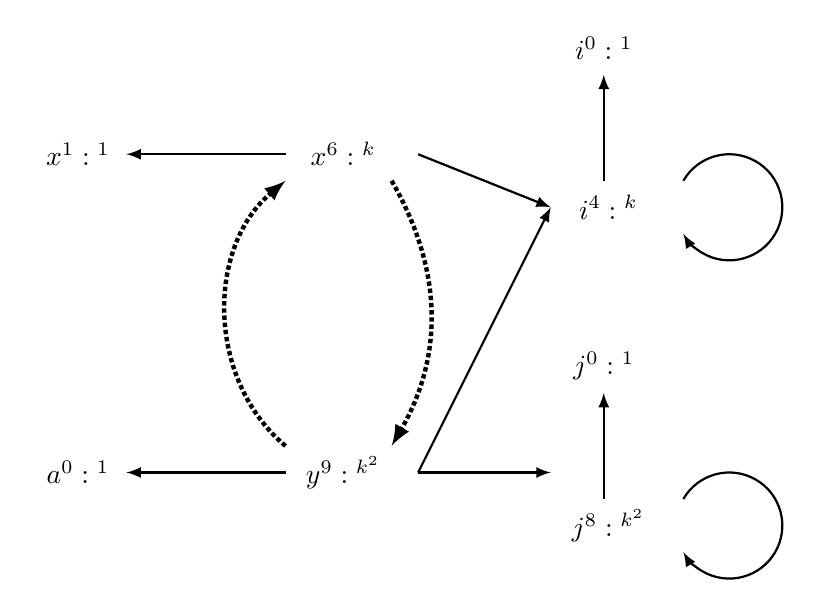
\begin{tikzpicture}[scale=\textwidth/18cm,samples=200]
      % Variables Initialization
      \draw[] (-5, 1) circle (0pt) node{{ $a^0: {}^1$}};
      \draw[] (-5, 7) circle (0pt) node{{ $x^1: {}^{1}$}};
      % Variables Inside the Loop
      \draw[] (0, 7) circle (0pt) node{{ $x^6: {}^{k}$}};
      \draw[] (0, 1) circle (0pt) node{{ $y^9: {}^{k^2}$}};
      % Counter Variables
      \draw[] (5, 9) circle (0pt) node {{$i^0: {}^{1}$}};
      \draw[] (5, 6) circle (0pt) node {{ $i^4: {}^{k}$}};
      \draw[] (5, 3) circle (0pt) node {{$j^0: {}^{1}$}};
      \draw[] (5, 0) circle (0pt) node {{ $j^8: {}^{k^2}$}};
      % Value Dependency Edges:
      \draw[ thick, -latex] (5, 6.5)  --       (5, 8.5) ;
      \draw[ thick, -latex] (5, 0.5)  --       (5, 2.5) ;
      % Value Dependency Edges on Initial Values:
      \draw[ thick, -latex,] (-1, 1)  -- (-4, 1) ;
      \draw[ thick, -latex,] (-1, 7)  -- (-4, 7) ;
      %
      \draw[ ultra thick, -latex, densely dotted,] (-1, 1.5)  to  [out=-220,in=220]  (-1, 6.5);
      % node[left]{\highlight{{$k$}}}
      \draw[ ultra thick, -latex, densely dotted,]  (1, 6.5) to  [out=-60,in=60] (1, 1.5) ;
      % node[right]{\highlight{{$k$}}}
      % Control Dependency
      \draw[ thick, -latex, ] (6.5, 6.5) arc (150:-150:1);
      \draw[ thick, -latex, ] (6.5, 0.5) arc (150:-150:1);
      \draw[ thick,-latex] (1.5, 7)  -- (4, 6) ;
      \draw[ thick,-latex] (1.5, 1)  -- (4, 6) ;
      \draw[ thick,-latex] (1.5, 1)  -- (4, 1) ;
   \end{tikzpicture}
   \caption{}
      \end{centering}
      \end{subfigure}
    }
     \caption{(a) Nested While Loop Example, (b) Execution-Based Dependency Graph, (c) The Static Program-Based Dependency graph.}
    \label{fig:heapcost_example.tex}
    \vspace{-0.5cm}
    \end{figure}
  \end{example}


% \section{The Joint Distribution as Non-Linear Property}
% \label{sec:generalcost-example}
% The following example in Example~\ref{ex:heapcost} shows that in general 
resource cost analysis, the $\THESYSTEM$  can give a better cost upper bound than the traditional 
data-flow or control-flow analysis.
% program shown in Figure~\ref{fig:heapcost_example.tex} shows the similarity
% between the adaptivity and cost estimation.
\begin{example}[Resource Cost Example]
  \label{ex:heapcost}
The example program shown in Figure~\ref{fig:heapcost_example.tex} shows the similarity
between the adaptivity and cost estimation.

In order to estimate the worst case heap cost in this program, I analyse the length 
of the list assigned to $x$ and $y$ in line:6 and line : 9 of this program, through $\THESYSTEM$.
Then,  $\THESYSTEM$ computes approximation
of heap resource cost by searching for longest finite walk.
\\
Specifically as follows, 
$\THESYSTEM$ first constructs the program-based execution as in Figure~\ref{fig:heapcost_example.tex},
with weight on each vertex. (The query annotation in the graph is omitted, which isn't useful in analysing the 
list length).
Then $\THESYSTEM$ compute the longest restricted finite walk on this graph.
\\
In order to compute the bound for heap resource cost, the length of walk takes the non-query vertices into consideration as 
well. 

%  largest length of $x$ and $y$ 
% search for a path: $y^6 \to y^6$, and compute the adaptivity for this path as 
% $k$.
% Notice here, another special operation I have in the second branch is Non-updating of
% % Non-updating the 
% $\kw{querynum}$ and $\kw{flowcapacity}$.
% This guarantees both the accuracy and the soundness.
% Specifically,
% % because a second visiting of the same vertex 
% if this vertex is visited, it indicates that a cycle is monitored and  
% % indicates there is a cycle goes back to this vertex, 
% the traversing on this cycle is finished by going back to this vertex.
% %
% % then, when 
% When I continuously search for walks heading out of this vertex, 
% the minimum weight on this cycle does not affect the walks going out of this vertex that not pass this cycle.
% However, if I keep recording the minimum weight, then we
% %  are restricting 
% restrict the visiting times of vertices on a walk by
% using the minimum weight of vertices not on this walk.
% %  , it is unsound anymore.
% Then, it is obviously that this leads to unsoundness.
% If I update the $\kw{flowcapacity}[y^6]$ as $k$ after visiting $y^6$ the second time 
% on this walk,
% % the walk $y^6 \to y^6$,
% and continuously visit $x^9$,
% then the $\kw{flowcapacity[k]}$ is 
% updated as $\min(k, k^2)$.
% So
% %  which 
% % restricting 
% the visiting times of $x^9$ is restricted by $k$ on the walk $y^6 \to y^6 \to x^9$.
% This restriction excludes the finite walk $y^6 \to y^6 \to x^9 \to x^9$ where $y^6$ and $x^9$ visited by $k^2$ times
% in the computation. 
% However, the finite walk $y^6 \to y^6 \to x^9 \to x^9$ where $y^6$ is visited $k$ times and $x^9$ $k^2$ times is 
% a qualified walk, and exactly the longest walk I aim to find. So, by Non-updating the $\kw{flowcapacity}$ after 
% visiting $y$ again, I guarantee that the visiting times og vertices on every searched walk will not be restricted by weights not on this walk,
% i.e., the soundness.
% \\
% In the last line of this dfs algorithm, line: 16, it returns the adaptivity heading out from its input vertex.
% \\
% By applying this deep first search strategy on every vertex on this SCC, 
% I compute the adaptivity of this SCC by taking the maximum 
% % adaptivity reaching every vertex on this SCC.
% value over every vertex.
%
As a result,
the largest heap resource consumed in total, by $y$ and $x$ together computed from the $\THESYSTEM$ is $1 + k^2 + k$.
Comparing to $k + k^2 + k^3$ estimated as  the longest weight path from traditional CFL-reachability method, 
$\THESYSTEM$ analysis result improves the accuracy by $O(n)$.

% Look at a Nested While Loop example program in Figure~\ref{fig:heapcost_example.tex}.
% Specifically,
% % because a second visiting of the same vertex 
% if this vertex is visited, it indicates that a cycle is monitored and  
% % indicates there is a cycle goes back to this vertex, 
% the traversing on this cycle is finished by going back to this vertex.
% %
% % then, when 
% When I continuously search for walks heading out of this vertex, 
% the minimum weight on this cycle does not affect the walks going out of this vertex that not pass this cycle.
% However, if I keep recording the minimum weight, then we
% %  are restricting 
% restrict the visiting times of vertices on a walk by
%  using the minimum weight of vertices not on this walk.
% %  , it is unsound anymore.
% Then, it is obviously that this leads to unsoundness.
 %
  %
  \begin{figure}
    \centering
    {
      % \footnotesize
    \begin{subfigure}{.4\textwidth}
    \begin{centering}
    % 
    $ 
    \begin{array}{l}
      \kw{nestedWhileMultiVarRecAcross}(k) \triangleq \\
      \clabel{\assign{i}{k} }^{0} ; 
      \clabel{ \assign{x}{[]}}^{1} ; 
      \clabel{ \assign{y}{[]}}^{2} ; \\
          \ewhile ~ \clabel{i > 0}^{3} ~ \edo ~ \\
          \Big(
           \clabel{\assign{i}{i-1}}^{4} ;
           \clabel{\assign{j}{k}}^{5} ;\\
           \clabel{\assign{x}{1::y} }^{6}  ; \\
           \ewhile ~ \clabel{j > 0}^{7} ~ \edo ~ \\
           \Big(
            \clabel{\assign{j}{j-1}}^{8};
            \clabel{\assign{y}{ 1::x }}^{9}
            \Big) \Big)
      \end{array}
    %       
    $
    \caption{}
    \end{centering}
    \end{subfigure}
    \quad
    \begin{subfigure}{.52\textwidth}
      \begin{centering}
      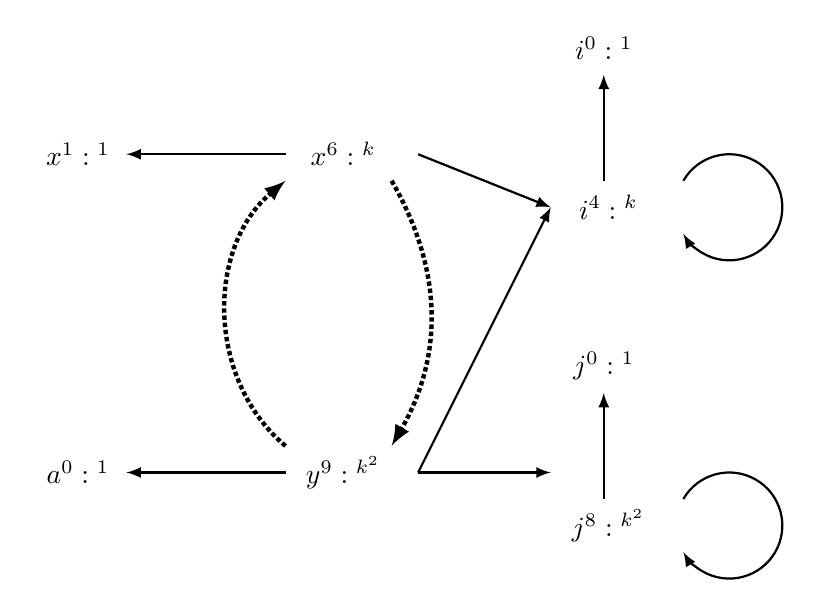
\begin{tikzpicture}[scale=\textwidth/18cm,samples=200]
      % Variables Initialization
      \draw[] (-5, 1) circle (0pt) node{{ $a^0: {}^1$}};
      \draw[] (-5, 7) circle (0pt) node{{ $x^1: {}^{1}$}};
      % Variables Inside the Loop
      \draw[] (0, 7) circle (0pt) node{{ $x^6: {}^{k}$}};
      \draw[] (0, 1) circle (0pt) node{{ $y^9: {}^{k^2}$}};
      % Counter Variables
      \draw[] (5, 9) circle (0pt) node {{$i^0: {}^{1}$}};
      \draw[] (5, 6) circle (0pt) node {{ $i^4: {}^{k}$}};
      \draw[] (5, 3) circle (0pt) node {{$j^0: {}^{1}$}};
      \draw[] (5, 0) circle (0pt) node {{ $j^8: {}^{k^2}$}};
      % Value Dependency Edges:
      \draw[ thick, -latex] (5, 6.5)  --       (5, 8.5) ;
      \draw[ thick, -latex] (5, 0.5)  --       (5, 2.5) ;
      % Value Dependency Edges on Initial Values:
      \draw[ thick, -latex,] (-1, 1)  -- (-4, 1) ;
      \draw[ thick, -latex,] (-1, 7)  -- (-4, 7) ;
      %
      \draw[ ultra thick, -latex, densely dotted,] (-1, 1.5)  to  [out=-220,in=220]  (-1, 6.5);
      % node[left]{\highlight{{$k$}}}
      \draw[ ultra thick, -latex, densely dotted,]  (1, 6.5) to  [out=-60,in=60] (1, 1.5) ;
      % node[right]{\highlight{{$k$}}}
      % Control Dependency
      \draw[ thick, -latex, ] (6.5, 6.5) arc (150:-150:1);
      \draw[ thick, -latex, ] (6.5, 0.5) arc (150:-150:1);
      \draw[ thick,-latex] (1.5, 7)  -- (4, 6) ;
      \draw[ thick,-latex] (1.5, 1)  -- (4, 6) ;
      \draw[ thick,-latex] (1.5, 1)  -- (4, 1) ;
   \end{tikzpicture}
   \caption{}
      \end{centering}
      \end{subfigure}
    }
     \caption{(a) Nested While Loop Example, (b) Execution-Based Dependency Graph, (c) The Static Program-Based Dependency graph.}
    \label{fig:heapcost_example.tex}
    \vspace{-0.5cm}
    \end{figure}
  \end{example}


% \section{Implementation}
% \label{sec:generalcost-implementation}

% Following the same system structure as $\THESYSTEM$,
% by modifying the restriction on finite walk, compute different resource cost for program.

